%%%%%%%%%%%%%%%%%%%%%%%%%%%%%%%%%%%%%%%%%%%%%%%%%%%%%%%%%%%%%%%%%%%%%%%%%%%%%%%%
%2345678901234567890123456789012345678901234567890123456789012345678901234567890
%        1         2         3         4         5         6         7         8

\documentclass[letterpaper, 10 pt, conference]{ieeeconf}  % Comment this line out if you need a4paper
\usepackage{dsfont,amssymb,amsmath, graphicx,fancyhdr,mdframed}
\usepackage[dvipsnames]{xcolor}
\usepackage{comment}
%% Tikz stuff
\usepackage{tikz}
\usetikzlibrary{arrows.meta} % Load arrows.meta for advanced arrow styles
\usetikzlibrary{fit, positioning}
\usetikzlibrary{calc}
\usetikzlibrary{decorations.pathmorphing} 

\tikzstyle{block} = [rectangle, minimum width=1cm, minimum height=1cm, text centered, draw=black]
\tikzstyle{tallblock} = [rectangle, minimum width=.5cm, minimum height=1cm, text centered, draw=black]
\tikzstyle{line} = [thick,-,>=stealth]
\tikzstyle{arrow} = [thick,->,>=stealth]
\tikzstyle{roundedblock} = [rectangle, minimum width=4cm, minimum height=2cm, text centered, draw=black, rounded corners=0.2cm]


\newcommand{\edit}[1]{\textcolor{blue}{#1}}
\newcommand{\emiliosay}[1]{\textcolor{ForestGreen}{[\textsc{Emilio:} #1]}}
\newcommand{\rezasay}[1]{\textcolor{DarkOrchid}{[\textsc{Reza:} #1]}}

\newcommand{\R}{\mathbb{R}}
\newcommand{\N}{\mathbb{N}}
\newcommand{\mc}{\mathcal}
\newcommand{\bs}{\boldsymbol}
\newcommand{\col}{\mathrm{col}}
\newcommand{\buol}{\boldsymbol{u}^{\mathrm{OL}}}
\newcommand{\uol}{u^{\mathrm{OL}}}
\newcommand{\Pol}{P^{\mathrm{OL}}}
\newcommand{\Kol}{K^{\mathrm{OL}}}
\newcommand{\Plqr}{P^{\mathrm{LQR}}}
\newcommand{\Klqr}{K^{\mathrm{LQR}}}
\newcommand{\bu}{\boldsymbol{u}}
\newcommand{\Dx}{D^{\text{x}}}
\newcommand{\Du}{D^{\text{u}}}
\newcommand{\dx}{d^{\text{x}}}
\newcommand{\du}{d^{\text{u}}}
\newcommand{\X}{\mathbb{X}}
\newcommand{\U}{\mathbb{U}}
\newcommand{\red}[1]{\textcolor{red}{#1}}
\newcommand{\VI}{\mathrm{VI}}
\newcommand{\tsum}{\textstyle\sum}
\newcommand{\blkdiag}{\mathrm{blkdg}}
\newcommand{\row}{\mathrm{row}}

\newcommand{\Ms}{M^{\mathrm{s}}}

\newtheorem{theorem}{Theorem}
\newtheorem{definition}[theorem]{Definition}
\newtheorem{lemma}[theorem]{Lemma}
\newtheorem{assumption}[theorem]{Assumption}
\newtheorem{remark}[theorem]{Remark}
\newtheorem{problem}{Problem}
\newtheorem{corollary}[theorem]{Corollary}
\newtheorem{fact}[theorem]{Fact}
\newtheorem{proposition}[theorem]{Proposition}
%\documentclass[a4paper, 10pt, conference]{ieeeconf}      % Use this line for a4 paper

\IEEEoverridecommandlockouts                              % 

\overrideIEEEmargins                                      % Needed to meet printer requirements.

%In case you encounter the following error:
%Error 1010 The PDF file may be corrupt (unable to open PDF file) OR
%Error 1000 An error occurred while parsing a contents stream. Unable to analyze the PDF file.
%This is a known problem with pdfLaTeX conversion filter. The file cannot be opened with acrobat reader
%Please use one of the alternatives below to circumvent this error by uncommenting one or the other
%\pdfobjcompresslevel=0
%\pdfminorversion=4

% See the \addtolength command later in the file to balance the column lengths
% on the last page of the document

% The following packages can be found on http:\\www.ctan.org
%\usepackage{graphics} % for pdf, bitmapped graphics files
%\usepackage{epsfig} % for postscript graphics files
%\usepackage{mathptmx} % assumes new font selection scheme installed
%\usepackage{times} % assumes new font selection scheme installed
%\usepackage{amsmath} % assumes amsmath package installed
%\usepackage{amssymb}  % assumes amsmath package installed

\title{\LARGE \bf
%Variational Inequalities in Dynamic Games:\\
%Snails, Turtles, or Cheetahs?
Douglas-Rachford Splitting Method for Solving \\
Monotone Variational Inequalities in Dynamic Games
}


\author{Reza Rahimi Baghbadorani, Emilio Benenati, Sergio Grammatico %<-this % stops a space
%\thanks{*This work was not supported by any organization}% <-
\thanks{The authors are with the Delft Center of Systems and
Control (DCSC), TU Delft, the Netherlands. E-mail addresses:
{\tt\small \{e.benenati, r.rahimibaghbadorani, s.grammatico\}@tudelft.nl}.}%
}


\begin{document}



\maketitle
\thispagestyle{empty}
\pagestyle{empty}


%%%%%%%%%%%%%%%%%%%%%%%%%%%%%%%%%%%%%%%%%%%%%%%%%%%%%%%%%%%%%%%%%%%%%%%%%%%%%%%%
\begin{abstract}
\rezasay{Emilio, It would be great if you could give your suggestions about the abstract.}
This paper considers linear dynamic games with quadratic objective functions. Building on previous results, we formulate the finite-horizon, constrained game as an affine variational inequality. Leveraging its structure, we incorporate it into the Douglas-Rachford splitting method to accelerate computation with a linear convergence guarantee. Additionally, we demonstrate that each corresponding variational inequality exhibits quadratic convergence when the timestep is sufficiently large. Finally, we benchmark the proposed method through numerical experiments in a \red{vehicle platooning application}.
\end{abstract}
%%%%%%%%%%%%%%%%%%%%%%%%%%%%%%%%%%%%%%%%%%%%%%%%%%%%%%%%%%%%%%%%%%%%%%%%%%%%%%%%
\section{Introduction}
Dynamic games provide a formal framework for analyzing multi-agent decision-making processes in dynamical systems, where agents' objectives and constraints are coupled through both the system dynamics and their performance criteria \cite{haurie2012games,suzanne2000dynamic,wang2022cooperative}. In such settings, each agent aims to optimize its own cost function while anticipating the actions of other agents, leading to strategic interactions that can be captured through various equilibrium concepts. Such frameworks have broad applications in systems and control \cite{fele2018framework}, including multi-robot systems \cite{hall2024game}, where agents must coordinate actions while avoiding conflicts, and autonomous transportation \cite{kada2020distributed}, where vehicles interact in mixed-autonomy traffic. In aerospace systems, dynamic games model strategic interactions in satellite coordination and pursuit-evasion scenarios \cite{musavi2017unmanned,li2020distributed}. These frameworks enable decentralized decision-making and the analysis of emergent behaviors in complex, multi-agent environments.\\
The desired solution concepts in dynamic games depend on the information structure assumed for the agents. One common approach is the open-loop Nash equilibrium (OL-NE), which defines a trajectory as a sequence of control inputs that is optimal for each agent, given the initial state and the input sequences chosen by the other agents \cite{monti2024feedback,sassano2021constructive}.
Recent work by \cite{benenati2024linear} demonstrates that the OL-NE can be interpreted as a Linear Quadratic Regulator (LQR) problem formulated in an augmented state space. In addition, the authors derive a new expression for the cost-to-go and show that \edit{the nominal trajectory of} a receding-horizon controller using this expression as the terminal cost \edit{achieves the infinite-horizon OL-NE.} Furthermore, the \edit{finite-horizon problem used to compute the receding-horizon input is shown equivalent to a variational inequality (VI).} However, the complexity of the derived VI can increase rapidly as the number of agents, \edit{the control horizon} and the number of constraints grows, which \edit{clashes with the fast online computation requirement.} This is where \red{the structure of the derived VI} can be leveraged to achieve faster convergence, which is the main contribution of this work. \emiliosay{I am not sure if we can say that we exploit the structure: all we do is using the linearity of the VI} \rezasay{I agree with you and change it to "the structure of the derived VI"} For this purpose, we review some algorithms for solving the VI problem, along with a simulation that highlights the contribution of this paper. Before proceeding, let us define the VI problem as follows:
\begin{equation}\label{VI-main}
\text{find} \,\, x^* \in \mathcal{C} \quad \textbf{s.t.} \, \inf\limits_{x\in \mathcal{C}}\langle F(x^*), x - x^* \rangle \geq 0,
\end{equation}
where $\mathcal{C}\subseteq\R^n$ is a \edit{closed, convex set, and $F:\R^n\rightrightarrows \R^n$ is a (in general set-valued) operator.} We assume that $F$ is monotone, locally Lipschitz, and the solution set of \eqref{VI-main} is nonempty. \red{Note that it is not difficult to see, using the first-order optimality condition, that one can rewrite \eqref{VI-main} as a monotone inclusion, $0 \in F + \mathcal{N}_{\mathcal{C}}(x)$, where $\mathcal{N}$ is the normal cone of the set \(\mathcal{C}\). This equivalence is beneficial and allows us to use splitting-type methods, as we see later}. Now, we are in the position to review some recent and closely related existing methods for solving \eqref{VI-main}:\\
%%%%%%%%%%%%%%%%%%%%%%%%%%%%%%%
\textbf{Projected Gradient Descent (PGD) \cite{nemirovskij1983problem}:}  
\emiliosay{Is this the actual name? $F$ might not be a gradient. I would call this Forward-Backward and point at e.g. \cite[\S 12.5.1]{facchinei2003finite}}\rezasay{Actually, in the optimization community, they call it GD because the operator acts as a gradient, but I think in the control community, people mostly call it FW.} \emiliosay{My concern remains: this is not a gradient }
\begin{align*}
    x^{k+1} &= \pi_{\mathcal{C}}(x^k - \lambda F(x^k)),
\end{align*}
where \(\lambda\) is the stepsize. This method guarantees convergence for strongly monotone operators (with constant \(\mu\)) and Lipschitz operators (with constant \(L\)) when \(\lambda \in (0, 2\mu/L^2)\).\\
\textbf{Extragradient Descent (ex-GD) \cite{malitsky2014extragradient}:} \emiliosay{Same comment as before. Is there a VI-solving analogous to the extragradient method?}\rezasay{Same as before, but I changed the reference to be more consistent.} 
\begin{align*}
    y^k &= \pi_{\mathcal{C}}(x^k - \lambda F(x^k)), \\
    x^{k+1} &= \pi_{\mathcal{C}}(x^k - \lambda F(y^k)),
\end{align*}
with \(\lambda\) as the stepsize. Unlike PGD, this method ensures convergence for Lipschitz operators (with constant \(L\)) when \(\lambda \in (0, 1/L)\). \\
\textbf{Nesterov's accelerated gradient descent (Nes-GD) \cite{nesterov2006solving}:}
\begin{align*}
    x^k &= \arg\max_{x \in \mathcal{C}} \, \sum_{i=0}^k \lambda_i \left[\langle F(y^i), y^i - x \rangle - \frac{\mu}{2} \|x - y^i\|^2\right], \\
    y^{k+1} &= \arg\max_{x \in \mathcal{C}} \, \langle F(x^k), x^k - x \rangle - \frac{\beta}{2} \|x - x^k\|^2,
\end{align*}
where \(\lambda_{k+1} = \frac{\mu}{L} \sum_{i=0}^k \lambda_i\) is the stepsize at iteration \(k+1\). This method guarantees convergence for strongly monotone operators (with constant \(\mu\)) and \(\beta = L\), where \(L\) is the Lipschitz constant of the operator \(F\).\\
\textbf{Projected Reflected Gradient Descent (PrjRef) \cite{malitsky2015projected}:}  
\begin{align*}
    x^{k+1} &= \pi_{\mathcal{C}}(x^k - \lambda F(2x^k - x^{k-1})),
\end{align*}
where \(\lambda\) is the stepsize. This method guarantees convergence for a Lipschitz operator (with constant \(L\)) when \(\lambda \in (0, (\sqrt{2}-1)/L)\). Unlike the extragradient method, it requires only one projection per iteration.\\
\textbf{Golden Ratio Algorithm (GRAAL) \cite{malitsky2020golden}:}  
\begin{align*}
    y^k &= (1-\beta)x^k + \beta y^{k-1}, \\
    x^{k+1} &= \pi_{\mathcal{C}}(y^k - \lambda F(x^k)),
\end{align*}
with \(\lambda\) as the stepsize and \(\beta \in \left(0, (\sqrt{5}-1)/2\right]\). This method ensures convergence for Lipschitz operators (with constant \(L\)) when \(\lambda \in (0, 1/(2\beta L))\) and requires one projection per iteration. Additionally, the stepsize can be chosen adaptively, leading to the Adaptive Golden Ratio Algorithm (aGRAAL) \cite{malitsky2020golden}: 
\begin{align*}
    \lambda_k &= \min\left\{(\beta + \beta^2)\lambda_{k-1}, \frac{\|x^k - x^{k-1}\|^2}{4\beta^2\lambda_{k-2}\|F(x^k) - F(x^{k-1})\|^2}\right\}.
\end{align*}
\textbf{Splitting type methods (DR-split) \cite{facchinei2003finite}:}\\
\red{In these types of methods, the operator \( F \) can be split into a summation of different operators. Then, solving \(\mathrm{VI}(\mathcal{C}, F)\) is equivalent to solving \(0 \in F_1 + F_2\), where \(F + \mathcal{N} = F_1 + F_2\)}, and the iterative update of each sub-operator leads to convergence towards the solution. A famous class of these algorithms is the Douglas-Rachford splitting method, which can be written as:
\begin{align*}
   y^{k+1} &= (I + \lambda F_2)^{-1}\left(x^k - \lambda F_1(x^k)\right), \\
   x^{k+1} &= x^k + \gamma(y^{k+1} - x^k),
\end{align*}
where $\gamma \in (0,2)$ is a relaxation parameter. The convergence of this method is guaranteed for different cases of $F_1$ and $F_2$; we refer interested readers to~\cite{giselsson2017tight,moursi1805douglas} for further details.

As shown in Section \ref{sec: OL-NE as VI}, the solution to the infinite OL-NE problem is equivalent to solving a sequence of strongly monotone affine variational inequality problems with linear constraints, i.e. $F = Mx + q$ and $\mathcal{C}: Dx \leq d$ (where $M$ can be a non-symmetric matrix). Therefore, having efficient methods to solve affine VIs is essential for addressing dynamic game problems (OL-NE). Figure \ref{fig1} presents a comparison of the residuals for the aforementioned methods applied to 10 randomly generated strongly monotone affine VIs, with a non-symmetric matrix $M \in \mathbb{R}^{n \times n}$, a vector $q \in \mathbb{R}^n$, and linear constraints defined by $D \in \mathbb{R}^{m \times n}$ and $d \in \mathbb{R}^{m}$, where $n = 100$ and $m = 20$.
\begin{figure}[!h]
     \centering
           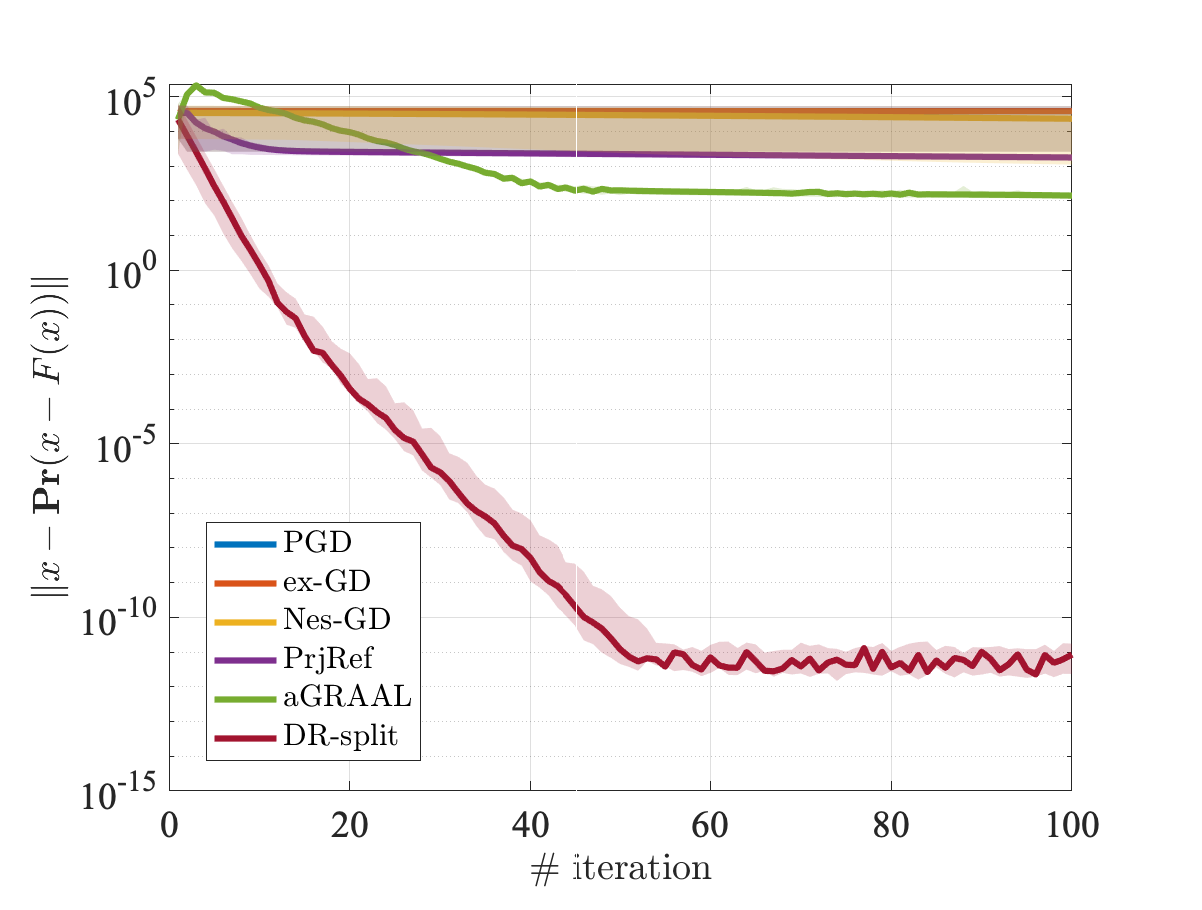
\includegraphics[width=0.45\textwidth]{VImethods.eps}
           \caption{Comparison of residuals for different variational inequality methods.}
           \label{fig1}
\end{figure}
As illustrated in Figure \ref{fig1}, the splitting method demonstrates superior performance compared to the other methods, which motivates leveraging the structure of the dynamical system to achieve faster convergence guarantees. With this in mind, our technical contributions are summarized as follows:
\begin{itemize}
   \item \textcolor{red}{First, we show how the infinite open-loop Nash equilibrium can be written as a successive strongly monotone affine VI with linear constraints. We also demonstrate that, over time, the solution of each VI becomes strictly feasible.}
   \item Second, we show how we can leverage the system dynamics in splitting-type methods to reduce the complexity and increase convergence. Furthermore, we guarantee linear convergence for the affine VI at each time step and also prove the quadratic convergence of VIs as the time step increases.
   \item Finally, we show the efficacy of the proposed splitting method in the \textcolor{red}{vehicle platooning} application through several numerical simulations.
\end{itemize}

\textit{\textbf{Notation.}} \rezasay{Emilio, please add the notation that you use in section \ref{sec: OL-NE as VI} and \ref{sec: simulation}}
Let $\mathcal{C}$ be the finite-dimensional real vector space with the standard inner product $\langle \cdot, \cdot \rangle$ and $\ell_p$-norm  $\|\cdot\|_p$ (by $\|\cdot\|$, we mean the Euclidean standard 2-norm).  We denote the $\pi_{\mathcal{C}}$ for the metric projection onto set $\mathcal{C}$ ($\pi_{\mathcal{C}}(x) = \arg\min_{y \in \mathcal{C}} \|x - y\|$). Operator $F$ is $L$-Lipschitz, if there is $L>0$ such that for all $x,y \in \mathcal{C}$ we have $\|F(x) - F(y)\| \leq L\|x-y\|$. The operator $F$ is monotone if $\langle F(x) - F(y), x - y \rangle \geq 0$ for all $x,y \in \mathcal{C}$ and it is called strongly monotone with constant $\mu > 0$ if 
$\langle F(x) - F(y), x - y \rangle \geq \mu \|x-y\|^2$ for all $x,y \in \mathcal{C}$.

\rezasay{I'm not sure if we need this part. We can remove it to save space.}\\
\textit{\textbf{Roadmap.}} In the rest of the paper, we first establish conditions to formulate the OL-NE as an affine VI problem in Section \ref{sec: OL-NE as VI}. Next, in Section \ref{sec:convergence}, we introduce a Douglas-Rachford splitting-type method to solve the derived VI linearly while ensuring quadratic convergence for each corresponding VI as the time steps increase. Section \ref{sec: simulation} benchmarks our proposed method through several experiments in a \red{vehicle platooning application}. Finally, discussions and future work are provided in Section \ref{sec: conclusion}.
%%%%%%%%%%%%%%%%%%%%%%%%%%%%%%%
\section{Open-Loop Nash equilibria as a VI}\label{sec: OL-NE as VI}
We consider a linear system with $N$ inputs, each controlled by a self-interest agent. We denote the sequence of control inputs of agent $i$ as $u_i$, and we denote time indexing with square brackets, for instance, $u_i[t]$ denotes the input at time index $t$. Define the set of agents $\mc I:=\{1,...,N\}$. We denote in boldface the stack over $\mc I$, for instance, $\bs{u}=(u_i)_{i\in\mc I}$, and in boldface with subscript $-i$ the stack over $\mc I \setminus \{i\}$, $\bs{u}_{-i}=(u_i)_{i\in\mc I \setminus \{i\}}$. The dynamics is ruled by the difference equation
\begin{equation}\label{eq:dynamics}
    x[t+1] = Ax[t] + \sum_{i\in\mc I} u_i[t].
\end{equation} 
We denote as $\phi(t, x_0, \bu)$ the solution at time $t$ of \eqref{eq:dynamics} with initial state $x_0$ and input $\bu$. We consider quadratic stage costs for all agents:
\begin{equation}
    \ell_i(x[t],u_i[t]):= x[t]^{\top}Q_ix[t] + u_i[t]^{\top}R_iu_i[t] \qquad \forall t
\end{equation}
and linear time-invariant constraints: define the stage-feasible sets as
\begin{align}
    \mathbb{U}_i(\bu_{-i}[t]):=\Large\{ u_i[t]: \sum_{j\in \mc I} \Du_j u_j[t] + \du &\leq 0 \Large\} \\
    \mathbb{X}:= \{x[t]: \Dx x[t]+ \dx \leq 0 \},
\end{align}
and the collective feasible input sequences with length $T\in\N\cup\{\infty\}$ as 
\begin{align}
        \mc{U}_T(x_0):= \large\{ \bu:~~ &u_i[t] \in \U_i(\bu_{-i}[t]) &\forall i,t; \\
         &\phi(t,x_0,\bu) \in\X &\forall t\large\}.
\end{align}
Note that, if $T$ is finite, $\mc U_T(x_0)$ can be expressed as a finite number of linear inequalities by substituting the dynamics to eliminate $\phi$: 
\begin{align}
    \bu&\in\mc U_T(x_0) \iff D\bu + d_{x_0} \leq 0, \label{def-constraint1}\\ 
    D &:= 
        \row\left(\begin{bmatrix}
            I_T \otimes \Du_i \\
            (I_T\otimes\Dx)\Gamma_i
        \end{bmatrix}\right)_{i\in\mc I} \label{def-constraint2}\\ 
    d_{x_0} &:= (I_T\otimes \Dx)\Theta x_0 \label{def-constraint3}\\
    \Theta &:= \col(A^k)_{k\in\{1,...,T\}}, \label{def-constraint4}\\
    \Gamma_i &:= \begin{bmatrix}
            B_i & 0 & \dots & 0 \\
            A B_i & B_i & \dots & 0 \\
            \vdots &  & \ddots & \\
            A^{T-1}B_i & A^{T-2}B_i & \dots  &B_i
        \end{bmatrix}. \label{def-constraint5}
\end{align}
We define the (infinite-horizon) Open-Loop Nash equilibrium (OL-NE) $\buol$ as an input sequence such that the infinite-horizon objective
\begin{equation}
    J_i(x_0, u_i, \bs{u}_{-i}):= \sum_{t=0}^{\infty} \ell_i\big(\phi(t,x_0,\bu),u_i[t]\big)
\end{equation}
cannot be improved by unilateral modifications by any agent. 
\begin{definition}[OL-NE] $\buol\in\mc{U}^{\infty}(x_0)$ is an OL-NE for the initial state $x_0$ if $\lim_{t\xrightarrow{}\infty} \phi(t,x_0,\buol)=0$ and
    \begin{equation}
        J_i^\infty(x_0, \uol_i, \buol_{-i})\leq J_i^\infty(x_0, u_i, \buol_{-i})
    \end{equation}
    for all $u_i$ such that $(u_i, \buol_{-i})\in\mc{U}^\infty(x_0)$.
\end{definition}
In \cite{benenati2024linear}, the authors determine a finite-horizon problem, whose solutions are a truncation of the OL-NE. Furthermore, this problem can be cast as a linear VI. We summarize these results next:
\begin{assumption} \label{as:objective_system}$Q_i=C_i^{\top}C_i \succeq 0$; $R_i = R_i^{\top}\succ 0$; the pairs $(A,B_i)$ and $(A,C_i)$ are respectively stabilizable and detectable for all $i$.
\end{assumption}
\begin{assumption}  \label{as:strict_feasibility} The origin is strictly feasible, that is,
    $0\in\mathrm{int}(\X)$; $\forall i: 0\in\mathrm{int}(\U_i(0))$.
\end{assumption}
\begin{assumption} \label{as:symplectic_matrix}
    $A$ is invertible and the matrix
    \begin{align*}
        H = \begin{bmatrix}
            A + \sum_{j\in\mc I}S_jA^{-\top}Q_j & \mathrm{row}(-S_jA^{-\top})_{j\in\mc I} \\
            \col(-A^{-\top}Q_j)_{j\in\mc I} & I_N \otimes A^{-\top}
        \end{bmatrix},
    \end{align*}
    where $S_i:=B_iR_i^{-1}B_i^{\top}$, has exactly $n$ eigenvalues with modulus strictly less than $1$. An $n$-dimensional invariant subspace of $H$ is complementary to
    \begin{equation*}
        \mathrm{Im}\left( \begin{bmatrix}0_{n\times Nn} \\ I_{Nn} \end{bmatrix} \right).
    \end{equation*}
\end{assumption}
The OL-NE is determined via the following procedure: \\
\emph{1)} Find $(\Pol_i, \Kol_i)_{i\in\mc I}$ that solve the coupled algebraic Riccati equations (ARE) \cite{freiling1999}
\begin{align}
    \Pol_i &= Q_i + A^\top\Pol_i(A +\tsum_{j\in\mc I}B_j \Kol_j) \\
    \Kol_i &= -R_i^{-1}B_i^{\top}\Pol_i(A +\tsum_{j\in\mc I}B_j \Kol_j);
\end{align}
\emph{2)} Find positive semi-definite $(\hat{P}_i)_{i\in\mc I}$ and $\hat{K}_i)_{i\in\mc I}$ that solve the (uncoupled) AREs 
\begin{subequations}
    \begin{align}
        \hat{P}_i &= \hat{Q}_i + \hat{A}_i^\top\hat{P}_i(\hat{A}_i+\hat{B}_i \hat{K}_i)\\
        \hat{K}_i &= -R_i^{-1}\hat{B}_i^{\top}\hat{P}_i(\hat{A}_i +\hat{B}_i \hat{K}_i),
    \end{align}
\end{subequations}
where 
\begin{align}
    \begin{split}
        \hat{A}_i &:= \begin{bmatrix}
        A & \tsum_{j\neq i} B_j \Kol_j \\
        0 & A + \tsum_{j\in\mc I} B_j \Kol_j
    \end{bmatrix}, \\
    \hat{Q}_i &:= \blkdiag(Q_i, 0_{n\times n}),\\
    \hat{B}_i &:= \col(B_i, 0_{n\times m}),
    \end{split}
\end{align}
\emph{3)} Solve the finite-horizon equilibrium problem
\begin{align} \label{eq:finite_hor_problem}
\begin{split}
\text{Problem $\mc P_1(x_0)$:}&~ \text{find $\bu^*\in\mc U(x_0)$ such that}\\ 
    \forall i: u_i^* \in \min_{u_i} &~~\sum_{t=0}^{T-1} \|\phi(t, x_0, u_i, \bu^*_{-i)})\|_{Q_i}^2 + \|u_i[t]\|^2_{R_i} \\ 
    &~~+\left\| \begin{bmatrix}
        \phi(T, x_0, u_i, \bu^*_{-i})\\
        \phi(T, x_0, \bu^*)
    \end{bmatrix} \right\|^2_{\hat{P}_i}\\
    \text{s.t.}&~~ (u_i, \bu^*_{-i})\in\mc U^T(x_0)
\end{split}
\end{align}
for some $T\in\N$. \\
Note that $\hat{P}_i\in\R^{2n\times 2n}$ and $\hat{K}_i\in\R^{m\times 2n}$. Consider the partition 
\begin{equation}
    \hat{K}_i = \begin{bmatrix}
        K_i^1 & K_i^2
    \end{bmatrix}
\end{equation}
with $K_i^1\in\R^{m\times n}$ and define 
\begin{equation}
    \Kol_i = K_i^1 + K_i^2 \quad \forall ~i.
\end{equation}
Let us introduce the ``terminal set'' $\X_f$ as a forward-invariant, constraint-admissible set for the dynamics 
$$x[t+1]=(A + \tsum_{j\in\mc I} B_j \Kol_j) x[t].$$

\begin{align} \label{eq:term_set}
\begin{split}
    \X_f:=\{x\in\mathrm{int}(\X): & 
    (A + \tsum_{i\in\mc I} B_i \Kol_i) x\in\X_f; \\
    &\tsum_{i\in \mc I}\Du_i\Kol_i x +\du <0
    \}.
\end{split}  
\end{align}
Note that this set is not enforced explicitly by a terminal constraint in \eqref{eq:finite_hor_problem}.
\begin{lemma}\cite[Theorem 1]{benenati2024linear}
    Let $\bu^*$ solve $\mc P_1(x_0)$, defined in \eqref{eq:finite_hor_problem}. Let $x_T:=\phi(T, x_0, \bu^*)$ and let $x_T\in \mathbb{X}_f$.
    Then, the sequence defined as
    \begin{equation}
        \forall i: \begin{cases}
            u_i^*[t] & \text{if} ~t < T,\\
            \Kol_i (A + \tsum_j B_j\Kol_j)^{t-T} x_T & \text{if} ~t\geq T
        \end{cases}
    \end{equation}
    is an OL-NE for the initial state $x_0$.
\end{lemma}
Intuitively speaking, if one defines the sequence of states and inputs
resulting from the linear feedback $(\Kol_j)_{j\in\mc I}$ 
\begin{align}\label{eq:unconstrained_NE_state_sequence}
    \phi^K(t,x_0)&:= (A + \tsum_i\in\mc I)^t x_0, & \forall ~i;\\
    u_i^K(t, x_0)&:= \Kol_i  \phi^{\text{ol}}(t,x_0), & \forall~i, t,
\end{align}
then the sequence $\bu^K(x_0)$ is a OL-NE for the unconstrained system. Furthermore, the function $\left\| \begin{bmatrix}
    x_0\\ y_0
\end{bmatrix} \right\|^2_{\hat{P}_i}$ identifies the $i$-th agent's optimal cost-to-go from state $x_0$, when the remaining agents apply the input sequence $\bu^K_{-i}(y_0)$ \cite[Lemma 1]{benenati2024linear}. 
% This is formalized in the following properties: We remand to \cite[\S 3B]{benenati2024linear} for their derivation.
% \begin{subequations}
%     \begin{align}
%         \left\|\begin{bmatrix}
%             x_0 \\ y_0
%         \end{bmatrix} \right\|_{\hat{P}_i} & \leq J_i^{\infty}(x_0, u_i, \bu^K_{-i}(y_0)) \\
%         \left\|\begin{bmatrix}
%             x_0 \\ x_0
%         \end{bmatrix} \right\|_{\hat{P}_i} &= J_i^{\infty}(x_0, u^K_i(x_0), \bu^K_{-i}(x_0)).
%     \end{align}
% \end{subequations}
Therefore, the terminal cost in \eqref{eq:finite_hor_problem} models the ``tail" of agent's $i$ objective for the terminal states $x[T]$ from which $u_i^K(x[T])$ is feasible, thus allowing one to compute the infinite-horizon constrained OL-NE via a finite-horizon problem. This  generalizes a known result in single-agent optimal control \cite{..}. We now link the solutions to $\mc P_1(x_0)$ to the solutions of a VI. Define the mapping 
\begin{equation} \label{eq:def_F}
        F(\bu, x_0) = M\bu + q,
    \end{equation}
    where
    \begin{align}\label{eq:def_VI_matrices}
    \begin{split}
        M&:= \mathrm{blkdg}(\bar{R}_i)_{i\in\mc I} + \begin{bmatrix}
            \Gamma_1^\top\bar{Q}_1\Gamma_1 & \dots &\Gamma_1^\top\bar{Q}_1\Gamma_N \\
            \Gamma_2^\top\bar{Q}_2\Gamma_1 & \dots & \Gamma_2^\top\bar{Q}_2\Gamma_N \\
            \vdots & \ddots & \\
            \Gamma_N^\top\bar{Q}_N\Gamma_1 & \dots & \Gamma_N^\top\bar{Q}_N\Gamma_1 
        \end{bmatrix}, \\
        q&:= \col(\Gamma_i^{\top}\bar{Q}_i\Theta x_0)_{i\in\mc I},\\
        \bar{R}_i&:= I_T\otimes R_i, \\
        \bar{Q}_i&:= \blkdiag(I_{T-1}\otimes Q_i, \Pol_i).
    \end{split}
    \end{align}

\begin{align}
\begin{split}
    &\text{Problem}~ \mc P_2(x_0): \text{find $\bu^*\in \mc U(x_0) $ such that} \\
    &\inf\limits_{\bu\in \mc U(x_0)}\langle F(\bu^*, x_0), \bu - \bu^* \rangle \geq 0,
\end{split}
\end{align}

\begin{lemma}\cite[Proposition 1?]{benenati2024linear}\label{lem: OL-NE as VI}
    If $\bu^*$ is a solution to $\mc P_2(x_0)$, then it is also a solution to  $\mc P_1(x_0)$.
\end{lemma}

\begin{figure}
    \centering
    \centering\resizebox{.7\columnwidth}{!}{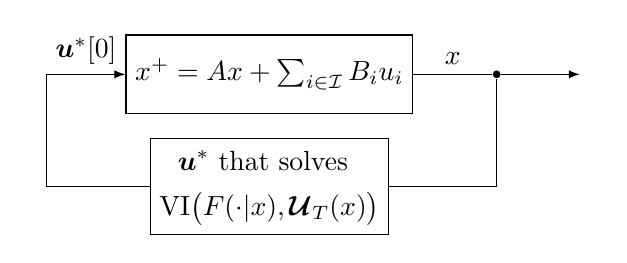
\begin{tikzpicture}[>=latex, node distance=1cm, auto]

    % Nodes
    \node [draw, block] (plant) at (0,0) {$x^+ = Ax + \tsum_{i\in\mc I} B_i u_i$};
    \node [draw, block, below=.3cmof plant] (GNEP) { $\begin{aligned}
        &~~\bu^* \text{ that solves} \\
        &\mathrm{VI}\big(F(\cdot|x), \bs{\mc U}_T(x)\big)
    \end{aligned}$ };

    \node [draw=none, left=of plant] (w) {};
    \node [fill=black, circle, right=of plant, inner sep=1pt] (dot) {};

    \node [draw=none, right=of dot] (x) {};

    % Connections

    \draw[-] (plant.east) --  node[above] {$x$}  (dot.west);
    \draw[-] (dot.south) |- (GNEP.east);
    \draw[->] (dot.east) -- (x.west);
    \draw[-] (GNEP.west) -| (w.east);
    \draw[->] (w.east) -- node[above] {$\bu^*[0]$}  (plant.west);
      
\end{tikzpicture}
}
    \caption{Receding-horizon OL-NE controller}
    \label{fig:block_scheme}
\end{figure}


Lemma \ref{lem: OL-NE as VI} identifies a computational method for the solutions of \eqref{eq:finite_hor_problem}, as efficient algorithms exist for the solution of a VI \cite{facchinei2003finite}. The need for a fast solution algorithm to $\mc P_2$ is of particular relevance, as the authors of \cite{benenati2024linear} propose the receding-horizon control action illustrated in Figure \ref{fig:block_scheme}, based on the recomputation at each timestep of its solution. With this application in mind, in the remainder of this paper, we explore a Douglas-Rachford (DR) splitting algorithm, which exploits the linear structure of the VI for its fast solution. This algorithm is linearly convergent \cite[Proposition 6]{ferris1996operator} when $M+M^{\top}\succ 0$, and it is advantageous compared to other commonly used VI solution methods, as illustrated in Figure \ref{fig1}.
\iffalse
\begin{lemma}
    If for all $i\in\mc I$
    \begin{align} \label{eq:gerschgorin_criterion}
    \begin{split}
    \lambda_{\text{min}}\left(\Gamma_i^{\top}\frac{\bar{Q}_i + \bar{Q}_i^{\top}}{2}\Gamma_i + \bar{R}_i\right) > \sum_{j\neq i} \left\| \Gamma_i^\top\frac{\bar{Q}_i+\bar{Q}_j^{\top}}{2}\Gamma_j \right\|,
    \end{split}
\end{align}
    and $\mc U_T(x_0)$ is non-empty, then $M+M^{\top}\succ 0$ and $VI(F(\cdot, x_0), \mc U_T(x_0))$ admits an unique solution for all $x_0$, where $F,M, (\bar{R}_i,\bar{Q}_i, \Gamma_i)_{i\in\mc I}$ are defined in \eqref{eq:def_F} and \eqref{eq:def_VI_matrices}.
\end{lemma}
\begin{proof}
$F$ admits a unique solution if $M+M^{\top}\succ 0$, following \cite[Proposition 2.3.2]{facchinei_finite-dimensional_2007}. Denote $\Ms = M + M^{\top}$ and consider its block partitioning with block size $Tm\times Tm$. Denote the $i,j$-th element as $\Ms_{i,j}$, with $i,j\in\mc I^2$. Clearly, $\Ms\succ 0$ if and only if $-\Ms$ is Hurwitz. From \cite[Corollary 2.34]{bullo_contraction_2024}, $-\Ms$ is Hurwitz if and only if its Metzler majorant \cite[\S 2.2]{bullo_contraction_2024}, denoted as $\lceil -\Ms \rceil$, is Hurwitz. By definition, 
\begin{equation}
    \lceil -\Ms \rceil = \begin{bmatrix} \mu(-\Ms_{11}) & \|\Ms_{12}\| & ... & \|\Ms_{1N}\| \\
        \|\Ms_{21}\| & \mu(-\Ms_{22}) & ... & \|\Ms_{2N}\| \\
        \vdots &  & \ddots & & \\
        \|\Ms_{N1}\| & \|\Ms_{N2}\| & ... & \mu(-\Ms_{NN}).
    \end{bmatrix}
\end{equation}
where $\mu(\cdot)$ denotes the $\ell_2$ induced log-norm \cite[Eq. 2.23]{bullo_contraction_2024}. Note that $\lceil -\Ms \rceil$ is symmetric, thus it is Hurwitz if and only if $-\lceil -\Ms \rceil\succ 0$. By the Gerschgorin disk theorem \cite[Theorem 2.8]{bullo_lectures_2024}, a sufficient condition is
\begin{equation} \label{eq:gerschgorin}
	-\mu(-\Ms_{ii}) \geq \sum_{j\neq i} \|\Ms_{ij}\| \qquad \forall i.
\end{equation}
From \cite[Example 2.25]{bullo_contraction_2024} and the matrix symmetry, it holds for all $i$ that $\mu(-\Ms_{ii}) = \lambda_{\text{max}}(-\Ms_{ii})$. Since $-\Ms_{ii}$ is negative definite, it holds that $\lambda_{\text{max}}(-\Ms_{ii}) = -\lambda_{\text{min}}(\Ms_{ii}) $. The statement immediately follows from \eqref{eq:gerschgorin}.
\end{proof}
In particular, \eqref{eq:gerschgorin_criterion} holds if $R_i=r_iI_m$, with $r_i>0$ large enough for all $i$. The resulting closed-loop system 
\begin{equation}\label{eq:closed_loop_dyn}
    x[t+1] = Ax[t] + \sum_{j\in\mc I} B_j \kappa_j(x[t]).
\end{equation}
is asymptotically stable, and its nominal dynamics is an infinite-horizon OL-NE following Lemma \ref{le:inf_hor_OLNE} and \cite[Lemma 2]{benenati2024linear}. 
\fi
 In Section \ref{sec:convergence}, we show its \red{quadratic} convergence when constraints are not active: This result is relevant in control applications, because the constraints are inactive in a neighborhood of the attractor following Assumption \ref{as:strict_feasibility}. Following the stability of the closed-loop system, one can expect the state to be in this region the majority of the time, under normal operating circumstances.
\begin{lemma}
    Let $x_0\in \mathbb{X}_f$. Let $M+M^{\top}\succ 0$. Let $\bu^*$ solve $\mc P_2(x_0)$. Then, $\bu^*\in\mathrm{int}(\mc U(x_0))$. 
\end{lemma}
\begin{proof}
    From the definition of $\mc U(x_0)$ and $\mathbb{X}_f$, the sequence $\bu^K(x_0)$ defined in \eqref{eq:unconstrained_NE_state_sequence}
    is strictly feasible. We show that $\bu(0:T-1, x_0)$ solves $\mc P_1(x_0)$. Consider a generic $T$-long sequence $v_i$. Proceeding by contradiction, we assume  
    \begin{equation}
        J_i(x_0, v_i, \bu^K_{-i}) < J_i(x_0,u_i^K,\bu_{-i}^K).
    \end{equation}
    Denote $x^v_T = \phi(T, x_0, v_i, \bu_{-i}^K)$ and $x^K_T = \phi(T, x_0, u_i^K, \bu_{-i}^K)$. 
    Following \cite[Lemma 1]{benenati2024linear} and the steps that lead to \cite[Eq. 21]{benenati2024linear}, the infinite sequence $w_i$ defined as
    \begin{equation}
        w_i[t]  = \hat{K}_i \left(\hat{A}_i + \begin{bmatrix}
            B_i \\0
        \end{bmatrix} \hat{K}_i\right)^t \begin{bmatrix}
            x_T^v \\ x_T^K
        \end{bmatrix} \quad \forall t\in\N
    \end{equation}
    achieves the infinite-horizon cost $\left\|\begin{bmatrix}
            x_T^v \\ x_T^K
        \end{bmatrix} \right\|^2_{\hat{P}_i}$, that is,
    \begin{equation}
        \left\|\begin{bmatrix}
            x_T^v \\ x_T^K
        \end{bmatrix} \right\|^2_{\hat{P}_i} = \sum_{t=0}^\infty \ell(\phi(t, x_T^v, w_i, \bu^K_{-i}(x_T^K)) , w_i[t] ).
    \end{equation}
    \begin{equation}
        v_i^\infty = \begin{cases}
            v_i[t] \\ 
            \begin{bmatrix}
                \Klqr_i & \Kol_i - \Klqr_i
            \end{bmatrix} \begin{bmatrix}
                A & \tsum_{j\neq i} B_j \Kol_j \\
                0 & A + \tsum_{j\in\mc I} B_j \Kol_j
            \end{bmatrix}
        \end{cases}
    \end{equation}
    
    Following \cite[Prop. 1]{benenati2024linear}, $\bu^K(x_0)$ is a unconstrained Nash equilibrium from $x_0$, thus for any sequence $v_i$ in $\R^m$,
    \begin{equation} \label{eq:uk_inf_hor_OLNE}
        J_i^{\infty} (x_0,  u_i^K, \bu_{-i}^K) \leq J_i^\infty (x_0, v_i, \bu^K_{-i}).
    \end{equation} In particular, \eqref{eq:uk_inf_hor_OLNE} holds for any $v_i$ such that 
    \begin{align}
        \sum_{t=T}^\infty \ell(\phi(t, x_0, v_i, \buol_{-i}), {u}_i[t]) = \left\|\begin{bmatrix}
            x_T^v \\ x_T^K 
        \end{bmatrix}\right\|^2_{\hat{P}_i}.
    \end{align}
    By contradiction, assume that there exists $v_i$ such that 
    Denote $x_v:= \phi(x_0,v_i, \bu^K_{-i}(x_0))$.
    \begin{align}\label{eq:cost_of_v}
        \begin{split}
            J_i(x_0, v_i, \bu^K_{-i}(x_0)) &= \tsum_{t=0}^{T-1} \ell(x_0, v_i, \bu^K_{-i}(x_0)) + \left\|[x^v, x^K] \right\|_{\hat{P}_i}\\
            & \leq \tsum_{t=0}^{T-1} \ell(x_0, v_i, \bu^K_{-i}(x_0)) + J_i^\infty(x^v, w_i, \bu^K_{-i}(x^K)) \\
            & = J_i^\infty(x_0, v_i^\infty, \bu^K_{-i})
        \end{split}
    \end{align}
    where the second inequality holds for any infinitely-long sequence of $\R^m$ $w_i$, and $v_i^\infty$ denotes the concatenation of $v_i$ and $w_i$. On the other hand,
    \begin{align}\label{eq:cost_of_u_K}
    \begin{split}
        J_i(x_0, u^K_i, \bu^K_{-i}) & = \sum_{t=0}^{T-1} \ell (\phi^K(t,x_0), u_i^K(t,x_0)) + \left\|\begin{bmatrix}
            \phi^K(T,x_0) \\ \phi^K(T,x_0)
        \end{bmatrix} \right\|_{\hat{P}_i} \\
        & \sum_{t=0}^{T-1} \ell (\phi^K(t,x_0), u_i^K(t,x_0)) + J_i^\infty(\phi^K(T,x_0), \bu^K(\phi^K(T,x_0))) \\
        & = J_i^\infty(x_0, \bu^K(x_0)).
    \end{split}
    \end{align}
\end{proof}
Comparing \eqref{eq:cost_of_v} and \eqref{eq:cost_of_u_K} leads to 
\begin{equation}
    
\end{equation}

%%%%%%%%%%%%%%%%%%%%%%%%%%%%%%%%%%%%%%%%%%%%%%%%%%%%%%%%%%%%%%%%%%%%%%%%%%%%%%%%
\section{Algorithm and Convergence}\label{sec:convergence}
In this section, based on the results from the previous section, we first establish linear convergence for the variational inequality at each time step in the OL-NE problem and also demonstrate quadratic convergence as the number of time steps increases. To this end, we consider the \(\mathrm{VI}(\mathcal{C}, F)\) corresponding to each time step in the OL-NE problem, as stated in Lemma \ref{lem: OL-NE as VI}, with the affine operator $F(u) = Mu + q$ and the constraint set $\mathcal{C}: Du + d_{x_0} \leq 0$, where $M$ and $q$ are defined in \eqref{eq:def_VI_matrices} and the set $\mathcal{C}$ is defined in \eqref{def-constraint1}-\eqref{def-constraint5}. Note that, based on the definition of $M$, we can choose the weight matrices $R_i$ such that the resulting operator is strongly monotone.\\
Now, we consider the following Douglas–Rachford splitting-type method to solve the mentioned affine VI, where $M$ can be expressed as a composition of two operators, $M_1$ and $M_2$:
\begin{subequations}\label{DR-affineVI}
\begin{align}
    y^{k} &= \text{sol}\left(H+M_1,\, q+(M_2 - H)u^k,\, \mathcal{C}\right), \label{DR-affineVI-1}\\
    u^{k+1} &= (H+M_2)^{-1}\left(H(2\lambda_k y^{k} + (1-2\lambda_k)u^k) + M_2u^k\right), \label{DR-affineVI-2}
\end{align}
\end{subequations}
where $H$ is an arbitrary symmetric positive definite matrix, and $\text{sol}\left(H + M_1,\, q + (M_2 - H)u^k,\, \mathcal{C}\right)$ denotes the solution to an affine variational inequality with operator $(H + M_1)u + q + (M_2 - H)u^k$ on the set $\mathcal{C}$.\\
The advantage of this splitting method is that if $M_1$ is a positive definite symmetric matrix and $H + M_2$ is invertible, then the iteration method in \eqref{DR-affineVI} is well-defined, and the iteration \eqref{DR-affineVI-1} is just a quadratic programming problem that can be computed efficiently. Fortunately, the dynamics of the OL-NE and the corresponding VI in Lemma \ref{lem: OL-NE as VI} provide us with the opportunity to choose the symmetric positive definite matrix $M_1$ and the positive semidefinite matrix $M_2$ (which is not necessarily symmetric) as follows, which satisfy the proposed properties.
\begin{align*}
    M_1 = \mathrm{blkdg}(\bar{R}_i)_{i\in\mc I}, \,\, M_2 = \begin{bmatrix}
            \Gamma_1^\top\bar{Q}_1\Gamma_1 & \dots &\Gamma_1^\top\bar{Q}_1\Gamma_N \\
            \Gamma_2^\top\bar{Q}_2\Gamma_1 & \dots & \Gamma_2^\top\bar{Q}_2\Gamma_N \\
            \vdots & \ddots & \\
            \Gamma_N^\top\bar{Q}_N\Gamma_1 & \dots & \Gamma_N^\top\bar{Q}_N\Gamma_1 
        \end{bmatrix},
\end{align*}
where $\bar{R}_i$, $\bar{Q}_i$, and $\Gamma_i$ are defined in \eqref{eq:def_VI_matrices}. The following lemma provides the linear convergence of the iterative method \eqref{DR-affineVI} for the affine VI, where $M$ can be written as $M = M_1 + M_2$.
\begin{lemma}\cite[Proposition 6]{ferris1996operator}\label{li-conv}
    \red{The residual of the affine \(\mathrm{VI}(\mathcal{C}, F)\) in the iterative method \eqref{DR-affineVI}, with the operator \( F = Mu + q \), where \( M \) can be expressed as \( M = M_1 + M_2 \), converges to zero linearly.}
\end{lemma}
\begin{proof}
   \red{As we assumed \( M_1 \) to be a positive definite matrix, it can be seen as a strongly monotone operator. Therefore, it is sufficient to consider case 2 in \cite[Proposition 6]{ferris1996operator}.}
\end{proof}
\begin{comment}
%\begin{proof}
  We use Theorem 6.5 from \cite{giselsson2017tight}, where the author proves the linear convergence rate of the Douglas-Rachford-type method \eqref{DR-affineVI} for finding the zero of the sum of two maximally monotone operators, i.e., $0 \ni T_1(x) + T_2(x)$, where $T_1(x)$ is a strongly monotone operator. \\
  By noting that solving the VI with operator $F$ on the set $\mathcal{C}$ is equivalent to solving $0 \ni F(x) + \mathcal{N}_\mathcal{C}(x)$, we deduce that the solution to \eqref{} satisfies $0 \ni M_1(x) + M_2(x) + q + \mathcal{N}_\mathcal{C}(x)$. Given the positive definiteness of $M_1$ and the maximal monotonicity of $M_2(x) + q + \mathcal{N}_\mathcal{C}(x)$, as stated in Proposition 1 of \cite{ferris1996operator}, and the linear convergence result from Theorem 6.5 in \cite{giselsson2017tight}, we can conclude the linear convergence of the residual VI \eqref{}.
%\end{proof}
\end{comment}
\red{We are now in a position to show a quadratic convergence of the corresponding VI in OL-NE at each time step as the number of time steps increases.}
\begin{theorem}[quadratic convergence]
   \red{The residual of affine \(\mathrm{VI}(\mathcal{C}, F)\) in the iterative method \eqref{DR-affineVI} with the strongly monotone operator $F = Mu + q$, associated with OL-NE at each time step, converges to zero quadratically as the number of time steps increases.}
\end{theorem}
\begin{proof}
   %The proof is straightforward. By applying Lemma \eqref{} we know that the solution is in the interior of the feasible set. Then, the problem reduces to solving a linear system of equations, $Mx + q \ni 0$. Now, by selecting a sufficiently small $H$ in the iterative method \eqref{DR-affineVI}, it becomes like Newton method for solving a linear system of equations which has at most quadratic complexity for strongly monotone VI \cite{taji1993globally,marcotte1987note}.
   \red{The proof is straightforward. By applying Lemma \eqref{lem: inactive cons}, we know that the solution of affine \(\mathrm{VI}(\mathcal{C}, F)\) lies in the interior of the feasible set $\mathcal{U}(x_0)$. Then, it is not difficult to see that the problem reduces to solving a linear system of equations, $0 \in Mu + q$. Now, by selecting a sufficiently small $H$ in the iterative method \eqref{DR-affineVI}, it becomes similar to the Newton method for solving a linear system of equations, which has a quadratic convergence \cite{greenbaum1997iterative}.}
\end{proof}
\red{We also refer interested readers to \cite{taji1993globally,marcotte1987note} where the authors use the Newton method to solve monotone VIs and show quadratic convergence for strongly monotone VIs in different scenarios.}
%%%%%%%%%%%%%%%%%%%%%%%%%%%%%%%%%%%%%%%%%%%%%%%%%%%%%%%%%%%%%%%%%%%%%%%%%%%%%%%%
\section{Numerical Experiments}\label{sec: simulation}
%%%%%%%%%%%%%%%%%%%%%%%%%%%%%%%%%%%%%%%%%%%%%%%%%%%%%%%%%%%%%%%%%%%%%%%%%%%%%%%%
\section{Conclusion and Future Directions}\label{sec: conclusion}

%%%%%%%%%%%%%%%%%%%%%%%%%%%%%%%%%%%%%%%%%%%%%%%%%%%%%%%%%%%%%%%%%%%%%%%%%%%%%%%%

\bibliographystyle{IEEEtran}
\bibliography{IEEEabrv, reference}

\end{document}
